% Real phone photos: apps v2.0.1 and v2.1.0. Every number is a macro from
% generated/realworld_numbers.tex, written by paper/make_tables.py; the figure
% comes from paper/make_scan_figure.py. Do not type results by hand.
The first release shipped the research model, and it failed on real photos.
This section describes the failure and the two changes that followed. The
research model and every result above are unchanged.

% Generated by paper/make_tables.py - do not edit
\begin{table}[t]
\centering
\caption{Classifiers at the gates the app used: the research model (shipped in v2.0.0) at its 95\%-validation gate, \ResGate{}; v2.0.1 at \GateVone{}; v2.1 at \GateVtwo{}. Upper rows: accepted with the right type; lower rows: accepted, where lower is better (\%, $n$ in brackets). v2.0.1 and v2.1 train on the training splits of both real-world sets, v2.1 also on COCO train2017 crops.}
\label{tab:clf}
\footnotesize
\setlength{\tabcolsep}{4pt}
\begin{tabular}{lccc}
\toprule
Test set & Research & v2.0.1 & v2.1 \\
\midrule
Web photos (60) & 13.3 & 45.0 & 53.3 \\
Fresh/rotten set, test (613) & 34.4 & 94.8 & 95.8 \\
Vegetable set, test (600) & 1.5 & 99.5 & 99.7 \\
Original grouped test (1,788) & 94.5 & 99.2 & 99.1 \\
External set (590) & 27.5 & 69.5 & 79.7 \\
COCO val2017 crops (574) & -- & 28.7 & 65.0 \\
\midrule
Unsupported produce, test (5,393) & 26.2 & 30.6 & 31.7 \\
CIFAR-10 (2,000) & 5.9 & 6.6 & 4.0 \\
\bottomrule
\end{tabular}
\end{table}
\begin{table}[t]
\centering
\caption{The whole app on real photos (\%). Right type: the best accepted item in the photo has the right type. Found: a detection matches the banana, apple or orange box one-to-one at IoU $\geq$ 0.5. AP50 is class-agnostic. False accept: at least one item accepted. COCO: the COCO-pretrained SSDlite, unchanged. $n$ in brackets.}
\label{tab:scan}
\footnotesize
\setlength{\tabcolsep}{3pt}
\begin{tabular}{lcccc}
\toprule
 & \multicolumn{2}{c}{Whole photo} & \multicolumn{2}{c}{Detector + crops} \\
\cmidrule(lr){2-3}\cmidrule(lr){4-5}
 & v2.0.1 & v2.1 & COCO & Ours \\
\midrule
\multicolumn{5}{l}{\textit{Right type}} \\
Web and user photos (62) & 45.2 & 53.2 & 67.7 & 72.6 \\
COCO single-type scenes (138) & 10.9 & 22.5 & 41.3 & 46.4 \\
\multicolumn{5}{l}{\textit{COCO val2017 fruit boxes (200 scenes)}} \\
Large (244), found & -- & -- & 59.0 & 55.7 \\
\quad found, right type & -- & -- & 38.9 & 38.9 \\
Medium (391), found & -- & -- & 6.1 & 11.3 \\
\quad found, right type & -- & -- & 4.3 & 8.2 \\
AP50, all produce & -- & -- & 22.1 & 20.7 \\
\multicolumn{5}{l}{\textit{False accepts (lower is better)}} \\
Unsupported produce (1,000) & 29.6 & 31.1 & 31.1 & 33.9 \\
CIFAR-10 (2,000) & 6.6 & 4.1 & 4.1 & 3.5 \\
\bottomrule
\end{tabular}
\end{table}


\begin{figure}[t]
\centering
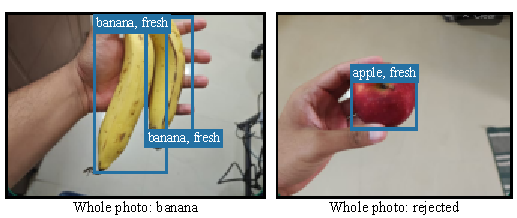
\includegraphics[width=\columnwidth]{figures/scan.pdf}
\caption{Our two phone photos through the v2.1 scan. Boxes: detections;
labels: type and freshness predicted for each crop, all accepted. Below each
photo: the v2.1 classifier on the whole photo.}
\label{fig:scan}
\end{figure}

\subsection{Web photos}
The released app (v2.0.0) rejected one of our own photos, bananas held in a
hand, as not a fruit. To see whether this was bad luck, we downloaded
\WebNRaw{} Creative Commons photos of the six supported types from Openverse,
labelled their type and freshness by eye and removed \WebNDup{} that nearly
duplicated a training image. No model is trained on the remaining \WebN{} web
photos. At its gate, the research model accepted \ResWebAccept\% of them and
named the type of \ResWebType\%, although it names the type of \ResMainType\% of its own test
images. On the test splits of two public sets of real-world photos, a
fresh/rotten set of fruit and vegetables~\cite{mukhiddinov2022fruitsveg} and a
vegetable set~\cite{ahmed2021vegetable}, the type was right for only
\ResFvType\% and \ResVegType\% of images. Our training photos show single items
on plain backgrounds from about \NSessions{} capture sessions, and a photo
taken in a kitchen looks different.

\subsection{A deployment model (app v2.0.1)}
We trained a second model for the app with the same multi-task
MobileNetV3-Large. It also learns from the training splits of the two
real-world sets; the vegetable set has no freshness labels, so its photos train
only the type head. Their photos of other produce form a new set of
unsupported produce, split in half, one half for choosing gates and the other
for testing. Augmentation is heavier than for the research model, with more
aggressive random crops, blur, JPEG recompression and stronger colour jitter.
At its own 95\%-validation gate the new model still rejected \DepValWebRej\% of
the web photos. Cluttered real photos and photos of unsupported produce get
similar energy scores, so no threshold separates them. We lowered the gate to
\GateVone{} after a sweep in which we looked at the web photos, which makes the
web results of v2.0.1 optimistic. Table~\ref{tab:clf} compares the classifiers
at the gates the app used.

\subsection{Why whole photos fail}
The next photo to fail showed one apple held in a hand over a floor
(Fig.~\ref{fig:scan}, right). The v2.0.1 app rejected it, and the v2.1
classifier described below rejects the whole photo too, but a square crop
around the apple passes the gate as an apple. The classifier had learned what a
photo looks like when one item fills the frame, and a cluttered photo does not
look like that. Crops of real scenes were still hard for it. Of \CocoCropsN{}
square crops around the annotated bananas, apples and oranges in COCO
val2017~\cite{lin2014coco}, v2.0.1 accepted only \VoneCocoCrops\% with the
right type. The app needed a way to find items, and the classifier needed to
see crops of real scenes.

\subsection{Two-stage scan (app v2.1.0)}
The app now finds each item first and classifies a square crop around it. The
detector is SSDlite from torchvision, with a MobileNetV3-Large
backbone~\cite{liu2016ssd,howard2019mobilenetv3}, pretrained on COCO. We replace
its COCO classifier with a single class, produce, initialised from COCO's
background and produce-class weights. With one class the detector only has to
find produce; whether an item is a supported type is left to the classifier and
its gate. The app keeps up to \DetMaxItems{} boxes that score at least
\DetScore{} after non-maximum suppression, cuts a square of \DetCropScale{}
times the longer box side around each, and classifies it. The score threshold
gives the best F1 at IoU 0.5 on validation (precision \DetValP, recall
\DetValR). If nothing is found, the app classifies the whole photo as before,
and users can also draw a box themselves.

\textbf{Detector data.} The detector trains on \DetNTrain{} images and is
validated on \DetNVal{}. They come from four sources: COCO train2017 scenes
with produce, using COCO's boxes for banana, apple, orange, broccoli and carrot
and Grounding DINO~\cite{liu2024groundingdino} boxes for produce that COCO has
no category for; food-free COCO scenes as negatives; photos from the three
Kaggle sets, boxed by Grounding DINO prompted with their known type; and
\DetNSynth{} synthetic scenes of SAM~\cite{kirillov2023sam} cutouts pasted onto
food-free COCO images, as in cut-and-paste
synthesis~\cite{dwibedi2017cutpaste,ghiasi2021copypaste}. A shape filter drops
masks that are slivers, fill nearly all of their box or have holes. We checked
small samples by eye: most automatic boxes were fully right and the rest partly
right, and the filter removed most faulty cutouts and none of the good ones.
None of the detector's data comes from COCO val2017, the web photos or the
classifier's test splits. AP50 on a fixed validation subset peaked at \DetValApFifty{} after epoch
\DetBestEpoch{} of \DetEpochs.

\textbf{Classifier v2.1.} We fine-tuned the v2.0.1 classifier for
\VtwoEpochs{} epochs on its own data plus \ClfNCrops{} crops cut the way the
app cuts them: \ClfNCoco{} around COCO train2017 boxes, with type labels only,
and \ClfNSynth{} from the synthetic scenes, with the type and, where the source
photo has one, the freshness label.

\textbf{Gates.} Both v2.1 gates were set on the validation half of the
unsupported produce, by matching false accepts. The whole-photo gate,
\GateVtwo, accepts the same share of these photos as v2.0.1 did at \GateVone.
Crops score higher than the photo they come from: at the whole-photo gate, the
detector's crops would accept \CalCropsAtWhole\% of \CalN{} validation photos,
against \CalWhole\% for whole photos. Crops therefore get their own gate, set
so that the two rates match. A photo counts as accepted when any of its items
passes.

\subsection{Results}
Fine-tuning on crops raised the share of COCO crops accepted with the right
type from \VoneCocoCrops\% to \VtwoCocoCrops\% (Table~\ref{tab:clf}). It also
helped on whole web photos and on the external set. The original test split
stayed at \VtwoMain\%, and fewer CIFAR-10 images passed the gate.

Table~\ref{tab:scan} compares whole apps. As a baseline for our detector we ran
the COCO-pretrained SSDlite unchanged, counting its banana, apple and orange
classes as produce, with a score threshold of \ProtoThr{} fixed in advance and
a crop gate calibrated in the same way. On the \ScanWebN{} web and user photos,
the best accepted item has the right type in \ScanWebVone\% of photos with the
v2.0.1 app, \ScanWebWhole\% with the v2.1 classifier on whole photos and
\ScanWebDet\% with the two-stage scan. On the \ScanSingleN{} COCO scenes that
contain a single supported type, the share rises from \ScanSingleVone\% to
\ScanSingleDet\%. When the type is right, the predicted freshness agrees with
our visual label on \ScanFreshDet\% of the \ScanFreshDetN{} web photos
concerned.

Items that fill little of the frame are the weak spot. SSDlite sees the photo
at \DetInput{}$\times$\DetInput{} pixels, and our detector finds
\ScanLargeFound\% of the large supported fruit in COCO scenes but only
\ScanMedFound\% of the medium-sized ones. Its class-agnostic AP50 over all annotated
produce is \ScanAp{}. That is a lower bound, because COCO does not annotate
tomatoes, peppers or lemons, and finding one counts as a false positive. The classifier loses
items too. Given the annotated boxes as crops, as a perfect detector would
supply them, it accepts the right type for \OracleLarge\% of large and
\OracleMed\% of medium fruit, so for medium fruit most of the loss is in
detection.

False accepts on unsupported produce went up. With both gates matched on
validation, the two-stage app accepts at least one item in \ScanOodDet\% of
\ScanOodN{} test photos of unsupported produce, against \ScanOodVone\% for
v2.0.1. On CIFAR-10, false accepts fall from \ScanCifarVone\% to
\ScanCifarDet\%.

On an Android emulator (profile build), the app's detector agreed with the
Python reference on \DevPhotos{} test photos: the same number of items in each
photo, \DevItems{} in all, with boxes within \DevBoxPx{} pixels and the same
type and gate decision for every item. On its own, the on-device classifier
matched PyTorch on type and gate for all \DevClfPhotos{} parity photos and on
freshness for \DevClfFresh{} of them. Median times
per photo were \DevDecodeMs{}\,ms to decode,
\DevDetectMs{}\,ms to detect and \DevCropsMs{}\,ms to classify all crops. The
detector's ONNX file is \DetOnnxMb{}\,MB.
